\documentclass{assignment}
\ProjectInfos{高等热力学与统计物理}{PHYS2110}{2020-2021学年第二学期}{习题 I}{截止时间:2021. . (周二)}{陈稼霖}{45875852}

\begin{document}
\begin{prob}
    令变量 $x$, $y$, $z$ 满足方程 $f(x,y,z)=0$,$w$ 为 $x$, $y$, $z$ 中任意两个变量的函数. 证明:
    \begin{itemize}
        \item[1)] $\left(\frac{\partial x}{\partial y}\right)_w\left(\frac{\partial y}{\partial z}\right)_w=\left(\frac{\partial x}{\partial z}\right)_w$
        \item[2)] $\left(\frac{\partial x}{\partial y}\right)_z\left(\frac{\partial y}{\partial x}\right)_z=1$
        \item[3)] $\left(\frac{\partial x}{\partial y}\right)_z\left(\frac{\partial y}{\partial z}\right)_x\left(\frac{\partial z}{\partial x}\right)_y=-1$
    \end{itemize}
    并用理想气体的状态方程验证 2) 和 3),其中 $x=P$, $y=T$, $z=V$.
\end{prob}
\begin{pf}
    \begin{itemize}
        \item[1)] 将 $w$ 写作 $x$, $y$ 的函数
        \begin{align}
            w=w(x,y)
        \end{align}
        并取微分,有
        \begin{align}
            \label{1-dw}
            \mathrm{d}w=\left(\frac{\partial w}{\partial x}\right)_y\mathrm{d}x+\left(\frac{\partial w}{\partial y}\right)_x\mathrm{d}y.
        \end{align}
        令上式中 $\mathrm{d}w=0$,得
        \begin{align}
            \label{1-(dx/dy)w}
            \left(\frac{\partial x}{\partial y}\right)_w=-\frac{\left(\frac{\partial w}{\partial y}\right)_x}{\left(\frac{\partial w}{\partial x}\right)_y}.
        \end{align}
        对式 $f(x,y,z)=0$ 取微分,有
        \begin{align}
            \label{1-df}
            \mathrm{d}f=\left(\frac{\partial f}{\partial x}\right)_{y,z}\mathrm{d}x+\left(\frac{\partial f}{\partial y}\right)_{x,z}\mathrm{d}y+\left(\frac{\partial f}{\partial z}\right)_{x,y}\mathrm{d}z=0,
        \end{align}
        从而可将 $\mathrm{d}x$ 表示为
        \begin{align}
            \mathrm{d}x=-\frac{\left(\frac{\partial f}{\partial y}\right)_{x,z}\mathrm{d}y+\left(\frac{\partial f}{\partial z}\right)_{x,y}\mathrm{d}z}{\left(\frac{\partial f}{\partial x}\right)_{y,z}}.
        \end{align}
        将上式代入式 \eqref{1-dw},得
        \begin{align}
            \mathrm{d}w=-\left(\frac{\partial w}{\partial x}\right)_y\frac{\left(\frac{\partial f}{\partial y}\right)_{x,z}\mathrm{d}y+\left(\frac{\partial f}{\partial z}\right)_{x,y}\mathrm{d}z}{\left(\frac{\partial f}{\partial x}\right)_{y,z}}+\left(\frac{\partial w}{\partial y}\right)_x\mathrm{d}y.
        \end{align}
        令上式中 $\mathrm{d}w=0$,得
        \begin{align}
            \label{1-(dy/dz)w}
            \left(\frac{\partial y}{\partial z}\right)_w=\frac{-\left(\frac{\partial w}{\partial x}\right)_y\left(\frac{\partial f}{\partial z}\right)_{x,y}}{\left(\frac{\partial w}{\partial x}\right)_y\left(\frac{\partial f}{\partial y}\right)_{x,z}-\left(\frac{\partial w}{\partial y}\right)_x\left(\frac{\partial f}{\partial x}\right)_{y,z}}.
        \end{align}
        由式 \eqref{1-df},也可将 $\mathrm{d}y$ 表为
        \begin{align}
            \mathrm{d}y=-\frac{\left(\frac{\partial f}{\partial x}\right)_{y,z}\mathrm{d}x+\left(\frac{\partial f}{\partial z}\right)_{x,y}\mathrm{d}z}{\left(\frac{\partial f}{\partial y}\right)_{x,z}}.
        \end{align}
        将上式代入式 \eqref{1-dw},得
        \begin{align}
            \mathrm{d}w=\left(\frac{\partial w}{\partial x}\right)_y\mathrm{d}x-\left(\frac{\partial w}{\partial y}\right)_x\frac{\left(\frac{\partial f}{\partial x}\right)_{y,z}\mathrm{d}x+\left(\frac{\partial f}{\partial z}\right)_{x,y}\mathrm{d}z}{\left(\frac{\partial f}{\partial y}\right)_{x,z}}.
        \end{align}
        令上式中 $\mathrm{d}w=0$ 得
        \begin{align}
            \label{1-(dx/dz)w}
            \left(\frac{\partial x}{\partial z}\right)_w=\frac{\left(\frac{\partial w}{\partial y}\right)_x\left(\frac{\partial f}{\partial z}\right)_{x,y}}{\left(\frac{\partial w}{\partial x}\right)_y\left(\frac{\partial f}{\partial y}\right)_{x,z}-\left(\frac{\partial w}{\partial y}\right)_x\left(\frac{\partial f}{\partial x}\right)_{y,z}}
        \end{align}
        式 \eqref{1-(dx/dy)w} 与 \eqref{1-(dy/dz)w} 相乘恰好等于式 \eqref{1-(dx/dz)w},
        \begin{align}
            \left(\frac{\partial x}{\partial y}\right)_w\left(\frac{\partial y}{\partial z}\right)_w=\frac{\left(\frac{\partial w}{\partial y}\right)_x\left(\frac{\partial f}{\partial z}\right)_{x,y}}{\left(\frac{\partial w}{\partial x}\right)_y\left(\frac{\partial f}{\partial y}\right)_{x,z}-\left(\frac{\partial w}{\partial y}\right)_x\left(\frac{\partial f}{\partial x}\right)_{y,z}}=\left(\frac{\partial x}{\partial z}\right)_w,
        \end{align}
        得证.
        \item[2)] 令 $z$ 保持不变,即在式 \eqref{1-df} 中令 $\mathrm{d}z=0$,得
        \begin{align}
            \mathrm{d}f=\left(\frac{\partial f}{\partial x}\right)_{y,z}\mathrm{d}x+\left(\frac{\partial f}{\partial y}\right)_{x,z}\mathrm{d}y=0,
        \end{align}
        从而
        \begin{align}
            \label{1-dx/dy}
            \left(\frac{\partial x}{\partial y}\right)_z=&-\frac{\left(\frac{\partial f}{\partial y}\right)_{x,z}}{\left(\frac{\partial f}{\partial x}\right)_{y,z}},\\
            \left(\frac{\partial y}{\partial x}\right)_z=&-\frac{\left(\frac{\partial f}{\partial x}\right)_{y,z}}{\left(\frac{\partial f}{\partial y}\right)_{x,z}}.
        \end{align}
        上面两式相乘,得
        \begin{align}
            \left(\frac{\partial x}{\partial y}\right)_z\left(\frac{\partial y}{\partial x}\right)_z=1.
        \end{align}
        \item[3)] 令式 \eqref{1-df} 中的 $\mathrm{d}x=0$ ,得
        \begin{align}
            \label{1-dy/dz}
            \left(\frac{\partial y}{\partial z}\right)_x=-\frac{\left(\frac{\partial f}{\partial z}\right)_{x,y}}{\left(\frac{\partial f}{\partial y}\right)_{x,z}}.
        \end{align}
        令式 \eqref{1-df} 中的 $\mathrm{d}y=0$,得
        \begin{align}
            \label{1-dz/dx}
            \left(\frac{\partial z}{\partial x}\right)_y=-\frac{\left(\frac{\partial f}{\partial x}\right)_{y,z}}{\left(\frac{\partial f}{\partial z}\right)_{x,y}}.
        \end{align}
        式 \eqref{1-dx/dy}, \eqref{1-dy/dz} 和 \eqref{1-dz/dx} 相乘,得
        \begin{align}
            \left(\frac{\partial x}{\partial y}\right)_z\left(\frac{\partial y}{\partial z}\right)_x\left(\frac{\partial z}{\partial x}\right)_y=-1.
        \end{align}
    \end{itemize}

    理想气体的状态方程为
    \begin{align}
        PV=nRT.
    \end{align}
    \emph{验证 2)}:
    \begin{align}
        &\left\{\begin{array}{l}
            \left(\frac{\partial P}{\partial T}\right)_V=\frac{nR}{V},\\
            \left(\frac{\partial T}{\partial P}\right)_V=\frac{V}{nR},
        \end{array}\right.\\
        \Longrightarrow&\left(\frac{\partial P}{\partial T}\right)_V\left(\frac{\partial T}{\partial P}\right)_V=1.
    \end{align}
    \emph{验证 3)}:
    \begin{align}
        &\left\{\begin{array}{l}
            \left(\frac{\partial P}{\partial T}\right)_V=\frac{nR}{V},\\
            \left(\frac{\partial T}{\partial V}\right)_P=\frac{P}{nR},\\
            \left(\frac{\partial V}{\partial P}\right)_T=-\frac{nRT}{P^2},
        \end{array}\right.\\
        \Longrightarrow&\left(\frac{\partial P}{\partial T}\right)_V\left(\frac{\partial T}{\partial V}\right)_P\left(\frac{\partial V}{\partial P}\right)_T=-\frac{nRT}{VP}=-1.
    \end{align}
\end{pf}

\begin{prob}
    假设热容量 $C_V$ 为常数,证明理想气体绝热过程中的下列关系:
    \begin{itemize}
        \item[1)] $PV^{\gamma}=$常数
        \item[2)] $TV^{\gamma-1}=$常数
        \item[3)] $PT^{\frac{\gamma}{1-\gamma}}=$常数
    \end{itemize}
    其中 $\gamma\equiv C_P/C_V$,并计算理想气体从初态 $(P_1,V_1)$ 到末态 $(P_2,V_2)$ 所做的功.
\end{prob}
\begin{sol}
    \begin{itemize}
        \item[1)] 由热力学第一定律,
        \begin{align}
            \label{2-Thermodynamics-1st-Law}
            \mathrm{d}U=\delta W+\delta Q
        \end{align}
        在绝热过程中,气体与外界无热量交换,$\delta Q=0$,而外界对气体所做的功为 $\delta W=-P\mathrm{d}V$. 对于理想气体,由焦耳定律知,内能的微分可表为 $\mathrm{d}U=C_V\,\mathrm{d}T$. 从而式 \eqref{2-Thermodynamics-1st-Law} 可化为
        \begin{align}
            \label{2-Thermodynamics-1st-Law-2}
            C_V\mathrm{d}T+P\,\mathrm{d}V=0.
        \end{align}
        将理想气体的物态方程 $PV=nRT$ 全式进行微分,得
        \begin{align}
            P\,\mathrm{d}V+V\,\mathrm{d}P=nR\,\mathrm{d}T.
        \end{align}
        由于定压热容 $C_P$ 和定容热容 $C_V$ 之差为 $C_P-C_V=nR$,上式可化为
        \begin{align}
            \label{2-d(PV=nRT)}
            P\,\mathrm{d}V+V\,\mathrm{d}p=(C_P-C_V)\,\mathrm{d}T=(\gamma-1)C_V\,\mathrm{d}T,
        \end{align}
        其中 $\gamma=C_P/C_V$. 联立式 \eqref{2-Thermodynamics-1st-Law-2} 和 \eqref{2-d(PV=nRT)},消去 $C_V$,得
        \begin{align}
            V\,\mathrm{d}P+\gamma P\,\mathrm{d}V=0,
        \end{align}
        即
        \begin{align}
            \frac{\mathrm{d}P}{P}=-\gamma\frac{\mathrm{d}V}{V}.
        \end{align}
        在温度变化范围较小的情况下,可将 $\gamma$ 视为常数,对上式积分,得
        \begin{align}
            \label{PV^gamma=const}
            PV^{\gamma}=\text{常数}.
        \end{align}
        \item[2)] 由理想气体的状态方程 $pV=nRT$,$P$ 可表为
        \begin{align}
            P=\frac{nRT}{V}.
        \end{align}
        将上式代入式 \eqref{PV^gamma=const},得
        \begin{align}
            TV^{\gamma-1}=\text{常数}.
        \end{align}
        \item[3)] 由理想气体的状态方程 $pV=nRT$,$V$ 可表为
        \begin{align}
            V=\frac{nRT}{P}.
        \end{align}
        将上式代入式 \eqref{PV^gamma=const},得
        \begin{align}
            P^{1-\gamma}T^{\gamma}=\text{常数}.
        \end{align}
        取上式的 $\frac{1}{1-\gamma}$ 次方,得
        \begin{align}
            pT^{\frac{\gamma}{1-\gamma}}=\text{常数}.
        \end{align}
    \end{itemize}

    理想气体从初态 $(P_1,V_1)$ 到末态 $(P_2,V_2)$ 对外界所做的功为
    \begin{align}
        W=\int_{V_1}^{V_2}P\,\mathrm{d}V=C\int_{V_1}^{V_2}\frac{\mathrm{d}V}{V^{\gamma}}=\frac{C}{\gamma-1}\left(\frac{1}{V_2^{\gamma-1}}-\frac{1}{V_1^{\gamma-1}}\right)
    \end{align}
    其中 $C$ 为常数,
    \begin{align}
        P_1V_1^{\gamma}=P_2V_2^{\gamma}=C.
    \end{align}
    故上式可化为
    \begin{align}
        W=\frac{P_2V_2-P_1V_1}{\gamma-1}.
    \end{align}
\end{sol}

\begin{prob}
    理想气体的 Carnot 循环:$A\rightarrow B\rightarrow C\rightarrow D\rightarrow A$\\
    --- 等温过程:$A\rightarrow B$(与高温热源接触)$C\rightarrow D$(与低温热源接触)\\
    --- 绝热过程:$B\rightarrow C$, $D\rightarrow A$.\\
    假设热容量为常数,证明循环效率为
    \[
        \eta=1-\frac{T_1}{T_2}.
    \]
    \begin{figure}[h]
        \centering
        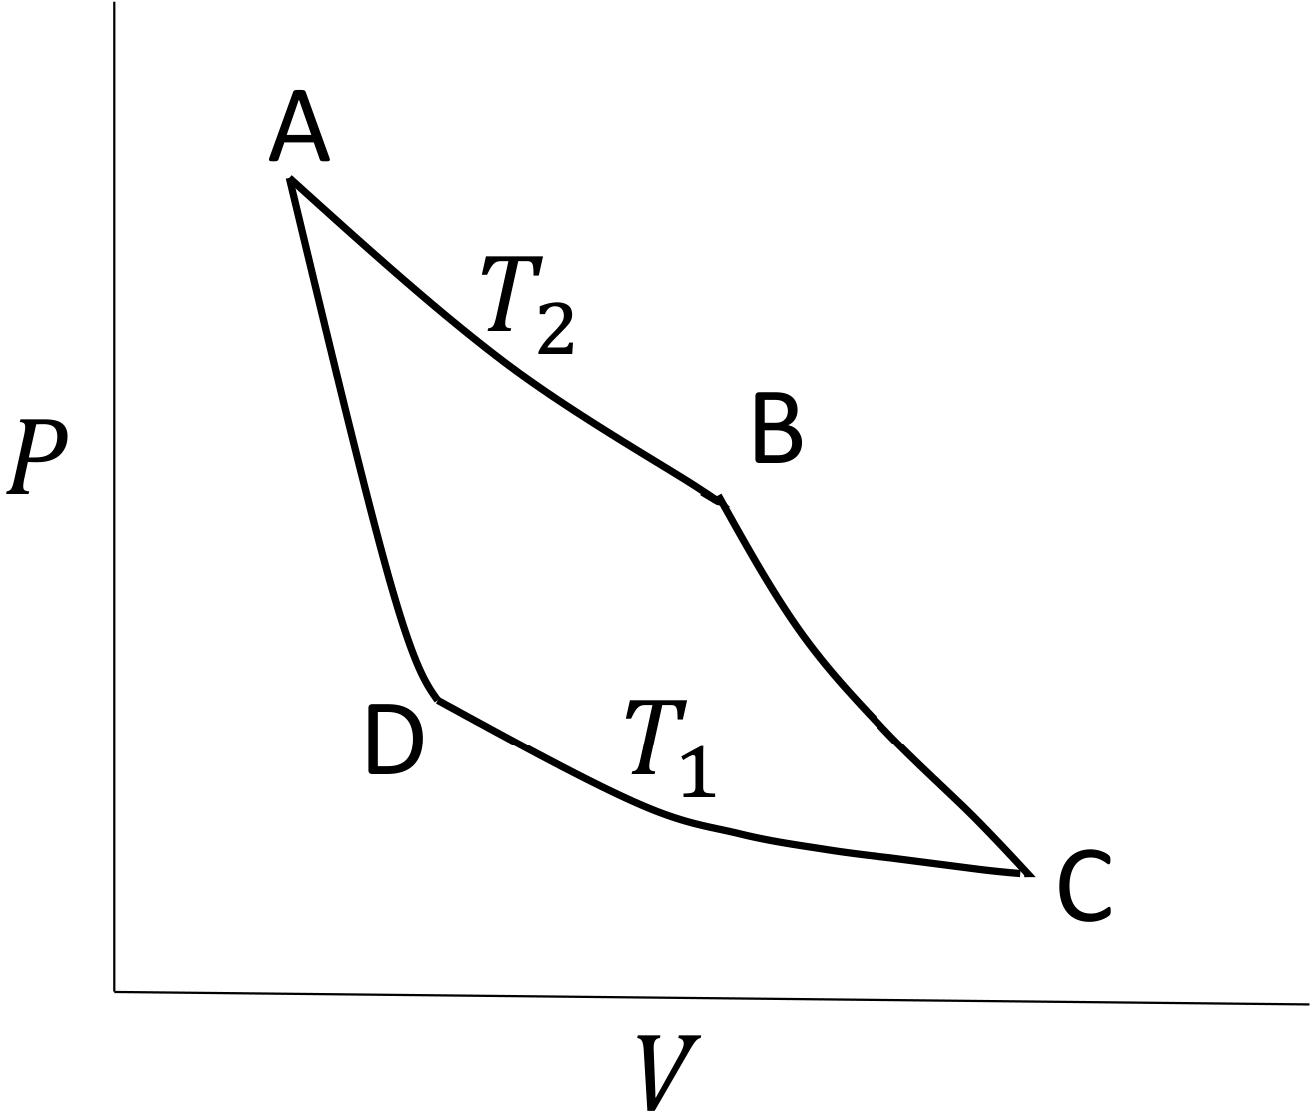
\includegraphics[width=.4\columnwidth]{A1-P3.png}
    \end{figure}
\end{prob}
\begin{pf}
    等温过程 $A\rightarrow B$ 中,外界对气体做的功为
    \begin{align}
        W_{A\rightarrow B}=-\int_{V_A}^{V_B}P\,\mathrm{d}V=-RT_1\int_{V_A}^{V_B}\frac{\mathrm{d}V}{V}=-RT_1\ln\frac{V_B}{V_A}.
    \end{align}
    等温过程中理想气体的内能不变,故由热力学第一定律可知,气体从高温热源吸收的热量为
    \begin{align}
        Q_1=-W_{A\rightarrow B}=RT_1\ln\frac{V_B}{V_A}.
    \end{align}
    同理,等温过程 $C\rightarrow D$ 中,气体向低温热源释放的热量为
    \begin{align}
        Q_2=RT_2\ln\frac{V_C}{V_D}.
    \end{align}
    绝热过程 $B\rightarrow C$ 和 $D\rightarrow A$ 中,气体与外界均无热量交换,因此,在一个 Carnot 循环中,气体净吸收的热量为
    \begin{align}
        Q=Q_1-Q_2=RT_1\ln\frac{V_B}{V_A}-RT_2\ln\frac{V_C}{V_D}.
    \end{align}
    一个 Carnot 循环后,气体回到原来的状态,故内能变化为零,由热力学第一定律知,在整个循环中,气体对外做的净功为
    \begin{align}
        W=Q=RT_1\ln\frac{V_B}{V_A}-RT_2\ln\frac{V_C}{V_D}.
    \end{align}
    因为过程 $B\rightarrow C$ 和 $D\rightarrow A$ 绝热,故有
    \begin{align}
        T_1V_B^{\gamma-1}=&T_2V_C^{\gamma-1},\\
        T_2V_D^{\gamma-1}=&T_1V_A^{\gamma-1}.
    \end{align}
    上面两式联立消去 $T_1$ 和 $T_2$,得
    \begin{align}
        \frac{V_B}{V_A}=\frac{V_C}{V_D}.
    \end{align}
    因此,
    \begin{align}
        W=R(T_1-T_2)\ln\frac{V_B}{V_A}.
    \end{align}
    在整个循环中,气体从高温热源吸收了热量 $Q_1$,对外做功 $W$,故循环效率为
    \begin{align}
        \eta=\frac{W}{Q_1}=\frac{R(T_1-T_2)\ln\frac{V_B}{V_A}}{RT_1\ln\frac{V_B}{V_A}}=1-\frac{T_2}{T_1}.
    \end{align}
\end{pf}
\end{document}